\section{Классификация}
\subsection{Общий подход к классификации через апостериорные вероятности} % (fold)
	Общая подход к классификации: строятся классифицирующие функции $f_i$, такие что классификация проводится так:
индивид с признаками $\mathbf{x}$ относится к группе с максимальным значением на нем классифицирующей функции:
$\argmax_i\mathrm f_i(\mathbf{x})$.

 Откуда берутся эти классифицирующие функции? Естественная идея взять в качестве $f_i$ вероятность (ее оценку)
принадлежности к $i$-му классу.
Пусть $\xi$ -- дискретная с.в., принимающая значения $\left\lbrace A_i\right\rbrace_{i=1}^k$, $\mathcal P(\eta\mid \xi = A_i) = \mathcal P_i$ и имеет плотность $p_i(\mathbf{x})$. Тогда было бы логично взять $f_i = p_i$. Для практического применения надо было бы оценить плотности, либо непараметрически (например, по числу точек, попавших в дельта-окрестность --- типа метода ближайших соседей), либо параметрически (если известно, что распределение нормальное, тогда просто оцениваем векторы средних и ковариационные матрицы).

Более сложный подход --- через апостериорные вероятности. Если у нас есть априорное знание вероятности того, что индивид
из того или иного класса, то мы можем его учесть.
Введем понятие класса $C_i = \left\lbrace\xi = A_i\right\rbrace$.  Чтобы классифицировать наблюдение $\mathbf{x}$, необходимо найти
	$$\argmax\mathrm P\left(\xi = A_i\middle\vert \eta = \mathbf{x}\right) = \argmax\mathrm P\left(C_i\middle\vert \mathbf{x}\right).$$

	Пусть известны априорные вероятности принадлежности нового наблюдения к $i$-му классу $\pi_i = \mathrm P\left(C_i\right)$. Тогда апостериорные вероятности по формуле Байеса будут иметь вид $$\mathrm P\left(C_i\middle\vert \mathbf{x}\right) = \frac{\mathrm P\left(\mathbf{x}\middle\vert C_i\right) \pi_i}{\sum_{j=1}^k \mathrm P\left(\mathbf{x}\middle\vert C_j\right) \pi_j}.$$
Поэтому в качестве классифицирующих функций берут
$$f_i\left(\mathbf{x}\right) = \frac{p_i(\mathbf{x}) \pi_i}{\sum_{j=1}^k p_j(\mathbf{x}) \pi_j}. $$

	Так как знаменатель у всех $f_i$ одинаковый, его можно отбросить, и итоговые классифицирующие функции будут выглядеть как $f_i\left(\mathbf{x}\right) = \mathrm P\left(\mathbf{x}\middle\vert C_i\right) \pi_i = p_i(\mathbf{x}) \pi_i$.

	Как выбрать априорные вероятности?

	\begin{enumerate}
		\item Равномерно, $\forall i \in 1\mathbin : k \; \pi_i = 1 \mathbin / k$.
		\item По соотношениям в обучающей выборке: $\pi_i = n_i \mathbin / \sum_{j=1}^k n_j$.
		\item На основе другой дополнительной информации о данных (результаты предыдущих исследований, etc.)
	\end{enumerate}

\begin{prop}
Построенный метод классификации $\mathrm{predict}(\mathbf{x}) = \argmax_i \pi_i p_i(\mathbf{x})$ минимизирует среднюю апостериорную ошибку:
$$\sum_{i=1}^k \pi_i \mathrm P(\mathrm{predict}(\mathbf{x}) != i\mid C_i).$$
\end{prop}

Видно, что можно с помощью априорных вероятностей формально задавать важность ошибочных классификаций
для разных классов.

%\end{document}
\subsection{Линейный и квадратичный дискриминантный анализ для классификации}
	\subsubsection{LDA} % (fold)
	\label{ssub:lda}
		Модель: $\xi$ --- дискретная с.в., принимающая значения $\left\lbrace A_i\right\rbrace_{i=1}^k$, $\mathcal P(\eta\mid \xi = A_i) = \mathcal N\left(\bm{\mu}_i, \bm{\Sigma}\right)$. Тогда плотность в точке $\mathbf{x}$
		$$p_i(\mathbf{x}) = p\left(\mathbf{x}\middle\vert \xi = A_i\right) = \frac{1}{\left(2\pi\right)^{p/2}\left\vert\bm{\Sigma}\right\vert^{1/2}} \exp\left(-\frac{1}{2}\Tr{\left(\mathbf{x} - \bm{\mu}_i\right)}\bm{\Sigma}^{-1}\left(\mathbf{x} - \bm{\mu}_i\right)\right),$$
		и классифицирующая функция $f_i\left(\mathbf{x}\right) = \pi_i p\left(\mathbf{x}\middle\vert \xi = A_i\right)$, где $\pi_i$ --- априорная вероятность наблюдения попасть в $i$-ю группу. Для упрощения вычислений можно переписать классифицирующую функцию через возрастающее монотонное преобразование как

		$$g_i\left(\mathbf{x}\right) = \log f_i\left(\mathbf{x}\right) = \log \pi_i - \frac{1}{2}\log\left\vert\bm{\Sigma}\right\vert -  \frac{1}{2}\Tr{\left(\mathbf{x} - \bm{\mu}_i\right)}\bm{\Sigma}^{-1}\left(\mathbf{x} - \bm{\mu}_i\right).$$
Сократив часть, не зависящую от номера класса, получаем линейные классифицирующие функции
$$h_i(\mathbf{x}) = -\frac{1}{2}\Tr{\bm{\mu}_i}\bm{\Sigma}^{-1}\bm{\mu}_i + \Tr{\bm{\mu}_i}\bm{\Sigma}^{-1}\mathbf{x} + \log\pi_i.$$

\begin{note}
  Если две группы, то гипотеза о равенстве многомерных мат.ож. $H_0: \bm{\mu}_1 = \bm{\mu}_2$ (различие значимо, если гипотеза отвергается, а только тогда имеет смысл проводить классификацию) в модели LDA проверяется с помощью критерия Хотеллинга (Hotelling). Если групп несколько, то есть разные критерии, например, критерия Wilk's Lambda или Roy's greatest root (эти же критерии используются в MANOVA, Multivariate ANalysis Of VAriance). Они отличаются мощностью против разного расположения групп.
\end{note}

\paragraph{Немного про канонические переменные}
В LDA есть так называемые канонические переменные. Идея похожа на АГК, только оптимизационная задача другая. Аналогично, на основе исходных признаков (признаки центрируются) строятся новые признаки как линейные комбинации исходных признаков. Только первая каноническая переменная --- это такая линейная комбинация исходных признаков, по которой группа максимально отличаются (отличие измеряется на основе ANOVA, по статистике критерия Фишера). Вторая линейная комбинация должна быть ортогональна первой и приводит к максимальному различию среди ортогональных линейных комбинаций. И т.д. Удобно смотреть на данные в плоскости первой и второй канонических переменных (иногда это называют roots).

\medskip
Приведем формулу, как находятся коэффициенты линейной комбинации (канонические коэффициенты) для получения канонических переменных. Неудивительно, что экстремальная задача приводит к поиску собственных векторов некоторой матрицы.

Имеет место разложение выборочной ковариационной матрицы, умноженной на $n$ (индивид $\mathbf y_{ij} \in \R^p$ --- $j$-й индивид из $i$-й группы):
\begin{gather}
    \label{VI_MANOVA}
    \sum_{i=1}^k \sum_{j=1}^{n_i} (\mathbf y_{ij} - \overline {\mathbf y}) \Tr{(\mathbf y_{ij} - \overline {\mathbf y})} =
    \sum_{i=1}^k n_i (\overline {\mathbf y_i} - \overline {\mathbf y}) \Tr{(\overline {\mathbf y_i} - \overline {\mathbf y})} +
    \sum_{i=1}^k \sum_{j=1}^{n_i} (\mathbf y_{ij} - \overline {\mathbf y_i}) \Tr{(\mathbf y_{ij} - \overline {\mathbf y_i})}
    = \mathbf{H}  + \mathbf{E}.
\end{gather}
Должно быть ясно, что это лишь многомерное обобщение разложения выборочной дисперсии (умноженной на $n$).

Первое слагаемое отвечает за равенство средних (неотличимые группы), его назовем $\mathbf{H}$ от слов hypothesis, а второе --- за отклонение данных в каждой группе от своего среднего, его назовем $\mathbf{E}$ от слова error.

В этих обозначениях, канонические коэффициенты являются собственными векторами матрицы $\mathbf{E}^{-1}\mathbf{H}$. А собственные числа $\lambda_i$ (упорядоченные по убыванию вместе с собственными векторами) этой матрицы отражают то, насколько группы хорошо разделяются по соответствующей канонической переменной. Число ненулевых собственных чисел $s\le \min(n, k-1)$.

Критерии для проверки гипотезы о том, что группы не разделимы ($H_0:\bm\mu_1=\ldots=\bm\mu_k$), являются комбинацией этих собственных чисел. Например, статистика критерия Wilks' Lambda $$\Lambda = \prod_{i=1}^s {\frac{1}{1 + \lambda_i}}$$ (с какой стороны критическая область?). А статистика критерия Roy's greatest root имеет вид $$r_1^2 = \frac{\lambda_1}{1+\lambda_1} $$ (с какой стороны критическая область?).

Как понять, против какого расположения группы мощнее один, а против какого --- другой?
	% subsubsection lda (end)

	\subsubsection{QDA} % (fold)
	\label{ssub:qda}

	Модель: $\xi$ --- дискретная с.в., принимающая значения $\left\lbrace A_i\right\rbrace_{i=1}^k$, $\mathcal P(\eta\mid \xi = A_i) = \mathcal N\left(\bm{\mu}_i, \bm{\Sigma}_i\right)$. Тогда плотность в точке $\mathbf{x}$
		$$p\left(\mathbf{x}\middle\vert \xi = A_i\right) = \frac{1}{\left(2\pi\right)^{p/2}\left\vert\bm{\Sigma}_i\right\vert^{1/2}} \exp\left(-\frac{1}{2}\Tr{\left(\mathbf{x} - \bm{\mu}_i\right)}\bm{\Sigma}_i^{-1}\left(\mathbf{x} - \bm{\mu}_i\right)\right),$$
		и классифицирующая функция $f_i\left(\mathbf{x}\right) = \pi_i p\left(\mathbf{x}\middle\vert \xi = A_i\right)$. Применяем возрастающее монотонное преобразование и оставляем в классифицирующей функции только члены, отличающиеся в разных группах:

		$$g_i\left(\mathbf{x}\right) = \log f_i\left(\mathbf{x}\right) = \log \pi_i - \frac{1}{2}\log\left\vert\bm{\Sigma}_i\right\vert -  \frac{1}{2}\Tr{\left(\mathbf{x} - \bm{\mu}_i\right)}\bm{\Sigma}_i^{-1}\left(\mathbf{x} - \bm{\mu}_i\right),$$
получаем квадратично зависящую от $\mathbf{x}$ классифицирующую функцию.

\begin{note}
  Если две группы, то гипотеза о равенстве многомерных мат.ож. $H_0: \bm{\mu}_1 = \bm{\mu}_2$ (различие значимо, если гипотеза отвергается, а только тогда имеет смысл проводить классификацию) в модели QDA тоже проверяется с помощью критерия Хотеллинга (Hotelling), но с отдельно оцененными ковариационными матрицами (критерий асимптотический). Если групп несколько, то тут уже критерий сложно построить.
\end{note}

\newpage
\subsection{Классификация в случае двух классов}
Если всего два класса, то можно построить границу между классами, приравняв классифицирующие функции.
\subsubsection{LDA} % (fold)
Приравняв $h_1(x)= h_2(x)$, получим разделяющую гиперплоскость.
Разделяющая два класса гиперплоскость имеет вид
\begin{multline*}
  \{\mathbf{x} : h_1(\mathbf{x}) = h_2(\mathbf{x})\} =\\ = \{\mathbf{x} : -\frac{1}{2} (\bm{\mu}_1 - \bm{\mu}_2)^\mathrm{T} \mathbf{\bm{\Sigma}}^{-1}(\bm{\mu}_1 + \bm{\mu}_2) + (\bm{\mu}_1 - \bm{\mu}_2)^\mathrm{T} \mathbf{\bm{\Sigma}}^{-1}\mathbf{x} + \log(\pi_1/\pi_2) = 0\}.
\end{multline*}
От соотношения между априорными вероятностями зависит положение границы относительно классов (к какому она ближе).
Видно, что априорные вероятности влияют только на сдвиг разделяющей гиперплоскости.

Заметим, что классификацию можно записать как сравнение $-\frac{1}{2} (\bm{\mu}_1 - \bm{\mu}_2)^\mathrm{T} \mathbf{\bm{\Sigma}}^{-1}(\bm{\mu}_1 + \bm{\mu}_2) + (\bm{\mu}_1 - \bm{\mu}_2)^\mathrm{T} \mathbf{\bm{\Sigma}}^{-1}\mathbf{x}$ с некоторым порогом ($-\log(\pi_1/\pi_2)$), который зависит от априорных вероятностей
(или весов ошибок для разных классов, смотря как на это смотреть).

\subsubsection{QDA} % (fold)
	В данном случае, разделяющая поверхность имеет вид квадратичной поверхности, может состоять из двух гиперболоидом,
может иметь форму эллипса.

\subsubsection{Картинки}

	\begin{figure}[!h]
		%\subfigure{
			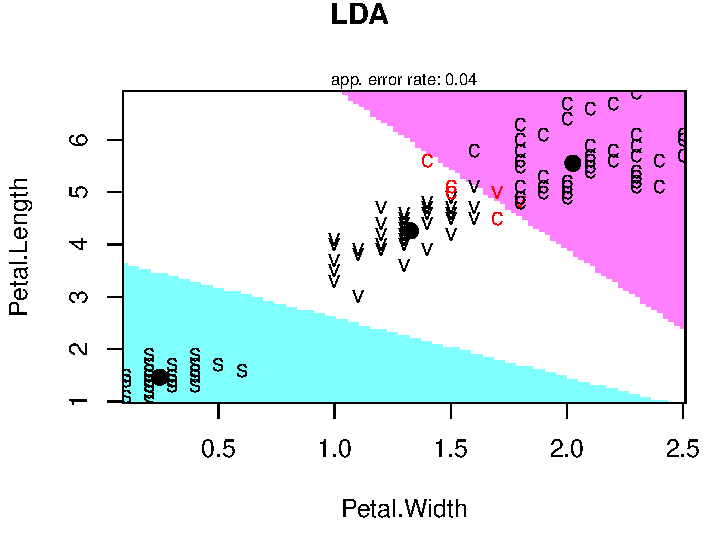
\includegraphics[width=0.5\textwidth]{img/lda.pdf}
			\includegraphics[width=0.5\textwidth]{img/qda.pdf}\\
			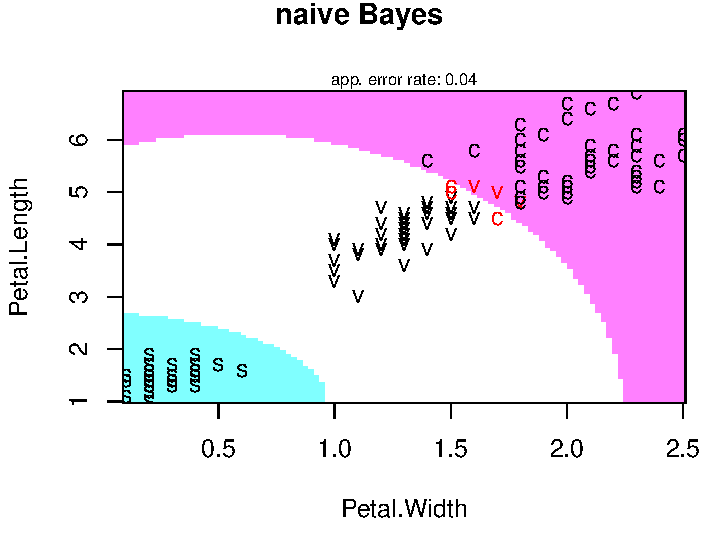
\includegraphics[width=0.5\textwidth]{img/nbda.pdf}
			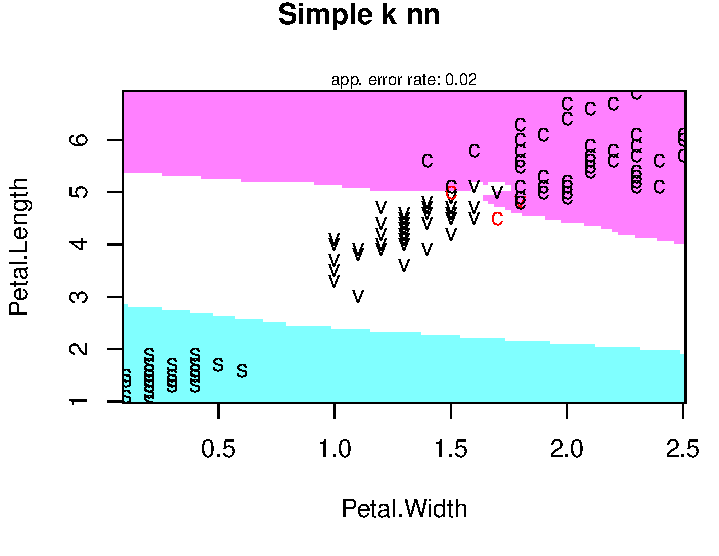
\includegraphics[width=0.5\textwidth]{img/sknn.pdf}
		%}
	\end{figure}

Здесь мы обсуждали число параметров в моделях, возможный overfitting (переподгонку).
Использовали слова --- обобщающая способность алгоритма.

\subsection{Качество классификации}


\subsubsection{Ошибки класификации}

Качество классификации измеряется ошибками классификации (доля неправильно классифицированных объектов).
$n_{ij}$ --- число объектов из класса $i$, отнесенных к классу $j$. В соответствующей матрице классификации
на диагонали стоят правильно классифицированные объекты, вне диагонали --- ошибки.

На самом деле, нельзя проверять качество предсказания на тех данных, на которых это предсказание строилось.
Поэтому используют кросс-валидацию (скользящий контроль).
Например, каждое наблюдение по очереди исключается из выборки, классифицирующее правило строится без него и с
 помощью этого правила индивид классифицируется. Строится аналогичная таблица из $n_{ij}$. В ней ошибок будет,
 вообще говоря, больше.

 Здесь обсуждали, что имеет смысл смотреть на ошибки без кросс-валидации и с ней. Если разница существенная, то
 это говорит о переподгонке используемой модели. Вероятно, она не очень хорошая; например, слишком много
 параметров.

Замечание. Нельзя путать классификацию и различие групп. Группы могут значимо различаться, классификация может
быть при этом бессмысленной
(ошибок чуть меньше 50\%).

\subsubsection{ROC и AUC}

\paragraph{wikipedia}

ROC-кривая (англ. receiver operating characteristic, рабочая характеристика приёмника) --- график, позволяющий оценить качество бинарной классификации, отображает соотношение между долей объектов от общего количества носителей признака, верно классифицированных как несущих признак, (англ. true positive rate, TPR, называемой чувствительностью алгоритма классификации) и долей объектов от общего количества объектов, не несущих признака, ошибочно классифицированных как несущих признак (англ. false positive rate, FPR, величина 1-FPR называется специфичностью алгоритма классификации) при варьировании порога решающего правила.

Также известна как кривая ошибок. Анализ классификаций с применением ROC-кривых называется ROC-анализом.

Количественную интерпретацию ROC даёт показатель AUC (англ. area under ROC curve, площадь под ROC-кривой) — площадь, ограниченная ROC-кривой и осью доли ложных положительных классификаций. Чем выше показатель AUC, тем качественнее классификатор, при этом значение 0,5 демонстрирует непригодность выбранного метода классификации (соответствует случайному гаданию). Значение менее 0,5 говорит, что классификатор действует с точностью до наоборот: если положительные назвать отрицательными и наоборот, классификатор будет работать лучше.

\paragraph{мои комментарии}

Если кто-то хорошо представляет себе, как выглядит график зависимости мощности от ошибки первого рода, то это именно такой график.
Меняется уровень значимости (как порог отвергнуть - не отвергнуть) и по оси x откладывается ошибка первого рода, она же false positive rate FP/(TN+FP), а по оси y откладывается
мощность, она же true positive rate TP/(TP+FN)(слово positive означает, что нулевая гипотеза отвергнута в пользу второй, альтернативной, гипотезы,
а в случае классификации, что элемент классифицируется как относящийся ко второму классу).

Таким образом, меняем порог/параметр для метода классификации (пример параметра --- априорная вероятность $\pi_1$)
и по оси x откладываем долю неправильно классифицированных элементов из первого класса ($n_{12}/(n_{11}+n_{12})$, FPR),
а по оси y --- долю правильно классифицированных элементов из второго класса ($n_{22}/(n_{22}+n_{21})$, TPR).

\includegraphics[width=10cm]{img/expl_roc}

Пусть классы имеют вид $4,6,8,10,12$ первый и $1,3,5,7$ второй. Опишем ROC-кривую. Пусть к первому классу мы относим, если число больше порога $\gamma$. Для $\gamma < 1$ мы находимся в точке $(0, 0)$. При $1 < \gamma < 3$ мы перескакиваем в точку $(0, 0.25)$. При $3 < \gamma < 4$ мы перескакиваем в точку $(0, 0.5)$. При $4 < \gamma < 5$ мы перескакиваем в точку $(0.2, 0.5)$. При $5 < \gamma < 6$ мы перескакиваем в точку $(0.2, 0.75)$.
При $6 < \gamma < 7$ мы перескакиваем в точку $(0.4, 0.75)$. При $7 < \gamma < 8$ мы перескакиваем в точку $(0.4, 1)$. Дальше мы при $x=1$ последовательно перескакиваем по $y$ в 0.6, 0.8 и при $\gamma >12$ попадаем в точку $(1,1)$.



%\end{document}
	% subsubsection qda (end)


% subsection _30_ (end)

	